%%%%%%%%%%%%%%%%%%%%%%%%%%%%%%%%%%%%%%%%%%%%%%%%%%%%%%%%%%%%%%%%%%%%%%%%
% Beamer Presentation - LaTeX - Template Version 1.0 (10/11/12)
% This template has been downloaded from: http://www.LaTeXTemplates.com
% License: % CC BY-NC-SA 3.0 (http://creativecommons.org/)
% Modified by Rahmat M. Samik-Ibrahim

% REV417: Sun 28 Jan 2024 16:00
% REV395: Sun 11 Sep 2022 22:00
% REV386: Thu 28 Jul 2022 13:00
% REV371: Mon 28 Feb 2022 10:00
% REV363: Mon 20 Dec 2021 15:00
% STARTX: Wed 14 Sep 2016 10:00
%%%%%%%%%%%%%%%%%%%%%%%%%%%%%%%%%%%%%%%%%%%%%%%%%%%%%%%%%%%%%%%%%%%%%%%%%

% PACKAGES AND THEMES 
\documentclass[aspectratio=169, xcolor=table, notheorems, hyperref={pdfpagelabels=false}]{beamer}
%%%%%%%%%%%%%%%%%%%%%%%%%%%%%%%%%%%%%%%%%%%%%%%%%%%%%%%%%%%%%%%%%%%%%%%%
% Beamer Presentation - LaTeX - Template Version 1.0 (10/11/12)
% This template has been downloaded from: http://www.LaTeXTemplates.com
% License: % CC BY-NC-SA 3.0 (http://creativecommons.org/)
% Modified by Rahmat M. Samik-Ibrahim
% REV419: Wed 24 Jul 2024 17:00
% REV383: Tue 12 Jul 2022 10:00
% REV316: Wed 14 Jul 2021 13:00
% REV198: Wed 13 Mar 2019 16:00
% REV005: Mon  2 Oct 2017 14:00
% STARTX: Thu 25 Aug 2016 14:00
%%%%%%%%%%%%%%%%%%%%%%%%%%%%%%%%%%%%%%%%%%%%%%%%%%%%%%%%%%%%%%%%%%%%%%%%%

%% ZCZC NNNN
\newtheorem{example}{Example}

%%%%%%%%%%%%%%%%%%%%%%%%%%%%%%%%%%%%%%%%%%%%%%%%%%%%%%%%%%%%%%%%%%%%%%%%%

\let\Tiny=\tiny
\mode<presentation> {
% The Beamer class comes with a number of default slide themes
% which change the colors and layouts of slides. Below this is a list
% of all the themes, uncomment each in turn to see what they look like.
%\usetheme{Boadilla}
\usetheme{Madrid}
% ZCZC %%%%%%%%%%%%%%%%%%%%%%%%%%%%%%%%%%%%%%%%%%%%%%%%%%%%%%%%%%%%%%%%%%
% \usetheme{default} \usetheme{AnnArbor} \usetheme{Antibes} \usetheme{Bergen}
% \usetheme{Berkeley} \usetheme{Berlin} \usetheme{CambridgeUS} 
% \usetheme{Copenhagen} \usetheme{Darmstadt} \usetheme{Dresden}
% \usetheme{Frankfurt} \usetheme{Goettingen} \usetheme{Hannover}
% \usetheme{Ilmenau} \usetheme{JuanLesPins} \usetheme{Luebeck}
% \usetheme{Malmoe} \usetheme{Marburg} \usetheme{Montpellier}
% \usetheme{PaloAlto} \usetheme{Pittsburgh} \usetheme{Rochester}
% \usetheme{Singapore} \usetheme{Szeged} \usetheme{Warsaw}
% NNNN %%%%%%%%%%%%%%%%%%%%%%%%%%%%%%%%%%%%%%%%%%%%%%%%%%%%%%%%%%%%%%%%%%
% As well as themes, the Beamer class has a number of color themes
% for any slide theme. Uncomment each of these in turn to see how it
% changes the colors of your current slide theme.
%\usecolortheme{orchid}
%\usecolortheme{rose}
%\usecolortheme{seagull}
%\usecolortheme{seahorse}
\usecolortheme{whale}
% ZCZC %%%%%%%%%%%%%%%%%%%%%%%%%%%%%%%%%%%%%%%%%%%%%%%%%%%%%%%%%%%%%%%%%%
%\usecolortheme{albatross} \usecolortheme{beaver} \usecolortheme{beetle}
%\usecolortheme{crane} \usecolortheme{dolphin} \usecolortheme{dove}
%\usecolortheme{fly} \usecolortheme{lily} \usecolortheme{wolverine}
% NNNN %%%%%%%%%%%%%%%%%%%%%%%%%%%%%%%%%%%%%%%%%%%%%%%%%%%%%%%%%%%%%%%%%%
% To remove the footer line in all slides uncomment this line
%\setbeamertemplate{footline} 
% To replace the footer line in all slides uncomment this line
%\setbeamertemplate{footline}[page number] 
% To remove the navigation symbols from the bottom uncomment this line
\setbeamertemplate{navigation symbols}{} 
}

\usepackage{array}       % ZCZC
\usepackage{amssymb}     % ZCZC
\usepackage{bold-extra}  % ZCZC
\usepackage{booktabs}    % Allows \toprule, \midrule and \bottomrule in tables
\usepackage{caption}
\usepackage[T1]{fontenc} % ZCZC << >>
\usepackage{graphicx}    % Allows including images
\usepackage{listings}    % listing
\usepackage{lmodern}     % ZCZC
\usepackage{perpage}     % reset footnote per page
\usepackage{geometry}    % ZCZC
\usepackage{adjustbox}   % ZCZC
\usepackage{multicol}    % ZCZC
\usepackage{multirow}    % ZCZC
\usepackage{pgf-pie}     % ZCZC pie chart

% \definecolor{links}{HTML}{2A1B81}
\definecolor{links}{HTML}{0011FF}
\hypersetup{colorlinks,linkcolor=,urlcolor=links}

% \usepackage{xcolor}
% \usepackage[colorlinks = true,
%             linkcolor = blue,
%             urlcolor  = blue,
%             citecolor = blue,
%             anchorcolor = blue]{hyperref}

\captionsetup[table]{name=Tabel}
\makeatletter
\def\input@path{{src/}}
\makeatother
\graphicspath{{src/}}      % src directory
\MakePerPage{footnote}     % reset page

% NNNN %%%%%%%%%%%%%%%%%%%%%%%%%%%%%%%%%%%%%%%%%%%%%%%%%%%%%%%%%%%%%%%%%%

%% % XXXXXXXXXXXXXXXXXXXXXXXXXXXXXXXXXXXXXXXXXXXXXXXXXXXXXXXXXXXXXXXXXXXXXXXXXX
%% % The short title appears at the bottom of every slide, 
%% % the full title is only on the title page
%% \title[Judul Pendek]{Judul Panjang dan Lengkap} 
%% \author{Cecak bin Kadal}
%% \institute[UILA]
%% {
%% University of Indonesia at Lenteng Agung \\ 
%% \medskip
%% \textit{cecak@binKadal.com}
%% }
%% \date{REV00 24-Aug-2016}
%% % \date{\today}
%% 

%% % XXXXXXXXXXXXXXXXXXXXXXXXXXXXXXXXXXXXXXXXXXXXXXXXXXXXXXXXXXXXXXXXXXXXXXXXXX
%% \begin{document}
%% \section{Judul}
%% \begin{frame}
%% \titlepage
%% \end{frame}
%% 
%% % XXXXXXXXXXXXXXXXXXXXXXXXXXXXXXXXXXXXXXXXXXXXXXXXXXXXXXXXXXXXXXXXXXXXXXXXXX
%% \section{Agenda}
%% \begin{frame}
%% \frametitle{Agenda}
%% % Throughout your presentation, if you choose to use \section{} and 
%% % \subsection{} commands, these will automatically be printed on 
%% % this slide as an overview of your presentation
%% \tableofcontents 
%% \end{frame}
%% 
%% % XXXXXXXXXXXXXXXXXXXXXXXXXXXXXXXXXXXXXXXXXXXXXXXXXXXXXXXXXXXXXXXXXXXXXXXXXX
%% \section{UUD dan Pancasila}
%% \subsection{UUD}
%% \begin{frame}
%% \frametitle{Pembukaan}
%% Bahwa sesungguhnya kemerdekaan itu ialah hak segala bangsa dan oleh 
%% sebab itu, maka penjajahan diatas dunia harus dihapuskan karena 
%% tidak sesuai dengan perikemanusiaan dan perikeadilan.
%% \\~\\
%% Atas berkat rahmat Allah Yang Maha Kuasa dan dengan didorongkan oleh 
%% keinginan luhur, supaya berkehidupan kebangsaan yang bebas, maka 
%% rakyat Indonesia menyatakan dengan ini kemerdekaannya.
%% \end{frame}
%% 
%% % XXXXXXXXXXXXXXXXXXXXXXXXXXXXXXXXXXXXXXXXXXXXXXXXXXXXXXXXXXXXXXXXXXXXXXXXXX
%% \begin{frame}
%% \frametitle{Alenia Ketiga}
%% Kemudian daripada itu untuk membentuk suatu pemerintah negara Indonesia 
%% yang melindungi segenap bangsa Indonesia dan seluruh tumpah darah Indonesia 
%% dan untuk memajukan kesejahteraan umum, mencerdaskan kehidupan bangsa, dan 
%% ikut melaksanakan ketertiban dunia yang berdasarkan kemerdekaan, perdamaian 
%% abadi dan keadilan sosial, maka disusunlah kemerdekaan kebangsaan Indonesia 
%% itu dalam suatu Undang-Undang Dasar negara Indonesia, yang terbentuk dalam 
%% suatu susunan negara Republik Indonesia yang berkedaulatan rakyat dengan 
%% berdasar kepada:
%% \begin{itemize}
%% \item Ketuhanan Yang Maha Esa,
%% \item kemanusiaan yang adil dan beradab,
%% \item persatuan Indonesia,
%% \item dan kerakyatan yang dipimpin oleh hikmat kebijaksanaan 
%%       dalam permusyawaratan/ perwakilan,
%% \item serta dengan mewujudkan suatu keadilan sosial bagi seluruh rakyat 
%%       Indonesia.
%% \end{itemize}
%% \end{frame}
%% 
%% % XXXXXXXXXXXXXXXXXXXXXXXXXXXXXXXXXXXXXXXXXXXXXXXXXXXXXXXXXXXXXXXXXXXXXXXXXX
%% \subsection{Pancasila}
%% \begin{frame}
%% \frametitle{Tujuh Kunci Pokok}
%% \begin{block}{Pertama - Kedua - Ketiga}
%% Indonesia ialah negara berdasarkan hukum.
%% Sistem konstitusional.
%% Kekuasaan negara tertinggi di tangan MPR.
%% \end{block}
%% 
%% \begin{block}{Keempat - Kelima}
%% Presiden adalah penyelenggara pemerintahan tertinggi di bawah MPR.
%% Adanya pengawasan DPR.
%% \end{block}
%% 
%% \begin{block}{Keenam}
%% Menteri negara adalah pembantu presiden dan tidak bertanggung jawab 
%% kepada DPR.
%% \end{block}
%% 
%% \begin{block}{Ketujuh}
%% Kekuasaan kepala negara tidak tak tebatas.
%% \end{block}
%% 
%% \end{frame}
%% 
%% % XXXXXXXXXXXXXXXXXXXXXXXXXXXXXXXXXXXXXXXXXXXXXXXXXXXXXXXXXXXXXXXXXXXXXXXXXX
%% \section{Rupa-rupa}
%% \subsection{Kolom}
%% \begin{frame}
%% \frametitle{Kolom}
%% % The "c" option specifies centered vertical alignment 
%% % while the "t" option is used for top vertical alignment
%% \begin{columns}[c] 
%% % Left column and width
%% \column{.45\textwidth} 
%% \textbf{Heading}
%% \begin{enumerate}
%% \item Satu-satu
%% \item Dua-dua
%% \item Tiga-tiga
%% \item Satu-dua-tiga
%% \end{enumerate}
%% 
%% % Right column and width
%% \column{.5\textwidth}
%% Satu-satu~\dots{} aku sayang ibu!
%% Dua-dua~\ldots{} juga sayang ayah!
%% Tiga-tiga~\ldots{} sayang adik kakak!
%% Satu-dua-tiga~\ldots{} sayang semuanya!
%% 
%% \end{columns}
%% \end{frame}
%% 
%% % XXXXXXXXXXXXXXXXXXXXXXXXXXXXXXXXXXXXXXXXXXXXXXXXXXXXXXXXXXXXXXXXXXXXXXXXXX
%% \subsection{Tabel}
%% \begin{frame}
%% \frametitle{Tabel}
%% \begin{table}
%% \begin{tabular}{l l l}
%% \toprule
%% \textbf{Nama} & \textbf{NPM} & \textbf{Tanggal Lahir}\\
%% \midrule
%% Cecak bin Kadal & 1234567890 & 1 Jan 2015 \\
%% Aneh bin Ajaib  & 0987654321 & 31 Des 2014 \\
%% \bottomrule
%% \end{tabular}
%% \caption{Keterangan Tabel}
%% \end{table}
%% \end{frame}
%% 
%% % XXXXXXXXXXXXXXXXXXXXXXXXXXXXXXXXXXXXXXXXXXXXXXXXXXXXXXXXXXXXXXXXXXXXXXXXXX
%% \subsection{Teori}
%% \begin{frame}
%% \frametitle{Teori}
%% \begin{theorem}[Teori Satu Batu]
%% $E = mc^2$
%% \end{theorem}
%% \end{frame}
%% 
%% % XXXXXXXXXXXXXXXXXXXXXXXXXXXXXXXXXXXXXXXXXXXXXXXXXXXXXXXXXXXXXXXXXXXXXXXXXX
%% \subsection{Verbatim}
%% % Need to use the fragile option when verbatim is used in the slide
%% \begin{frame}[fragile] 
%% \frametitle{Verbatim}
%% \begin{example}[Teori Satu Batu]
%% \begin{verbatim}
%% \begin{theorem}[Teori Satu Batu]
%% $E = mc^2$
%% \end{theorem}
%% \end{verbatim}
%% \end{example}
%% \end{frame}
%% 
%% % XXXXXXXXXXXXXXXXXXXXXXXXXXXXXXXXXXXXXXXXXXXXXXXXXXXXXXXXXXXXXXXXXXXXXXXXXX
%% \subsection{Gambar}
%% \begin{frame}
%% \frametitle{Gambar}
%% \begin{figure}
%% \includegraphics[width=0.5\linewidth]{2}
%% \caption{Ini Gambar JPG}
%% \end{figure}
%% \end{frame}
%% 
%% % XXXXXXXXXXXXXXXXXXXXXXXXXXXXXXXXXXXXXXXXXXXXXXXXXXXXXXXXXXXXXXXXXXXXXXXXXX
%% \subsection{Rujukan}
%% % Need to use the fragile option when verbatim is used in the slide
%% \begin{frame}[fragile] 
%% \frametitle{Rujukan dan Kutipan}
%% Contoh penggunaan \verb|\cite| ketika mengutip\cite{p1}.
%% Perhatian: Beamer tidak mengerti \verb|\BibTeX|~\ldots
%% \footnotesize{
%%   \begin{thebibliography}{99} 
%%   \bibitem[Smith, 2012]{p1} John Smith (2012)
%%      \newblock Katak dalam Tempurung
%%      \newblock \emph{Jurnal Kelapa dan Amfibi} 12(3), 45 -- 678.
%%   \end{thebibliography}
%% }
%% \end{frame}
%% 
%% % XXXXXXXXXXXXXXXXXXXXXXXXXXXXXXXXXXXXXXXXXXXXXXXXXXXXXXXXXXXXXXXXXXXXXXXXXX
%% \subsection{Selesai}
%% \begin{frame}
%% \Huge{\centerline{Selesai}}
%% \end{frame}
%% 
%% % XXXXXXXXXXXXXXXXXXXXXXXXXXXXXXXXXXXXXXXXXXXXXXXXXXXXXXXXXXXXXXXXXXXXXXXXXX
%% \end{document}

\newcommand{\revision}{%
REV426: Wed 13 Nov 2024 04:00
}
% w! tmptmp
% REV426: Wed 13 Nov 2024 04:00
% REV419: Wed 24 Jul 2024 17:00
% REV409: Tue 08 Aug 2023 12:00
% REV399: Fri 03 Feb 2023 20:00
% REV339: Sat 04 Sep 2021 12:00
% STARTS: Wed 24 Aug 2016 19:00
%%%%%%%%%%%%%%%%%%%%%%%%%%%%%%%%%%%%%
\newcommand{\kopikopi}{\textcopyright{}2016-2024 CBKadal + VauLSMorg}



% XXXXXXXXXXXXXXXXXXXXXXXXXXXXXXXXXXXXXXXXXXXXXXXXXXXXXXXXXXXXXXXXXXXXXXXXXX
% The short title appears at the bottom of every slide, 
% the full title is only on the title page
% \date{\today}
\title[\kopikopi]
{CSGE602055 Operating Systems \\ 
CSF2600505 Sistem Operasi \\
Week 10:
I/O \& Programming}
\author{C. BinKadal}
\institute[SdnBhd]
{
Sendirian Berhad\\
\medskip
\url{https://docOS.vlsm.org/Slides/os10.pdf}
\\ \texttt{Always check for the latest revision!}
}
\date{\revision}

% XXXXXXXXXXXXXXXXXXXXXXXXXXXXXXXXXXXXXXXXXXXXXXXXXXXXXXXXXXXXXXXXXXXXXXXXXX
\begin{document}

\lstset{
basicstyle=\ttfamily\tiny, % \tiny \small \footnotesize 
breakatwhitespace=true,
language=C,
columns=fullflexible,
keepspaces=true,
breaklines=true,
tabsize=3, 
showstringspaces=false,
extendedchars=true}

\section{Start}
\begin{frame}
\titlepage
\end{frame}

% XXXXXXXXXXXXXXXXXXXXXXXXXXXXXXXXXXXXXXXXXXXXXXXXXXXXXXXXXXXXXXXXXXXXXXXXXX

%%%%%%%%%%%%%%%%%%%%%%%%%%%%%%%%%%%%%%%%%%%%%%%%%%%%%%%%%%%%%%%%%%%%%%%%%
% REV418: Tue 30 Jan 2024 22:00
% REV406: Sat 05 Aug 2023 14:00
% REV399: Thu 02 Feb 2023 00:00
% REV369: Mon 14 Feb 2022 09:00
% REV328: Sat 14 Aug 2021 06:00
% STARTX: Wed 14 Sep 2016 10:00
%%%%%%%%%%%%%%%%%%%%%%%%%%%%%%%%%%%%%%%%%%%%%%%%%%%%%%%%%%%%%%%%%%%%%%%%%

\begin{frame}[fragile]
\section{OS241 Schedule}
\frametitle{OS241\footnote{%
) This information will be on \textbf{EVERY} page two (2) of this course material.}): 
Operating Systems Schedule 2023 - 2}

\vspace{5pt}

\scalebox{0.99}{%
\begin{tabular}{|c|c|l|l|}
\hline
\textbf{Week} & 
\textbf{Topic}\footnote{%
) For schedule, see \url{https://os.vlsm.org/\#idx02}}) & \textbf{OSC10}\footnote{%
    ) Silberschatz et. al.: \textbf{Operating System Concepts}, $10^{th}$ Edition, 2018.}) \\
\hline
Week 00  & Overview (1), Assignment of Week 00           & Ch. 1, 2      \\
Week 01  & Overview (2), Virtualization \& Scripting     & Ch. 1, 2, 18. \\
Week 02  & Security, Protection, Privacy, \& C-language. & Ch. 16, 17.   \\
Week 03  & File System \& FUSE  & Ch. 13, 14, 15.                        \\
Week 04  & Addressing, Shared Lib, \& Pointer & Ch. 9. \\
Week 05  & Virtual Memory & Ch. 10. \\
\hline
Week 06  & Concurrency: Processes \& Threads & Ch. 3, 4. \\
Week 07  & Synchronization \& Deadlock & Ch. 6, 7, 8. \\
Week 08  & Scheduling + W06/W07 & Ch. 5. \\
Week 09  & Storage, Firmware, Bootloader, \& Systemd & Ch. 11. \\
Week 10  & I/O \& Programming & Ch. 12. \\%
% MidTerm  & 00 XXX 2020 (XX:XX-XX:XX) & MidTerm (UTS) & \cellcolor{red!44} TBA! \\
% Reserved & 00 XXX - 00 XXX 2020 & Q \& A & \\
% Final    & 00 XXX 2020 XX:XX & First Part Final  (UAS tahap I)  & \cellcolor{red!44} This schedule is   \\
% Extra    & NA & No Extra assignment & \cellcolor{red!44} subject to change. \\
\hline
\end{tabular}
}
\end{frame}

\begin{frame}[fragile]
\frametitle{\textbf{STARTING POINT} --- 
{
\definecolor{links}{HTML}{FDEE00}
\hypersetup{colorlinks,linkcolor=,urlcolor=links}
\url{https://os.vlsm.org/}
}
}
\begin{itemize}
\item[$\square$] \textbf{Text Book} ---
                 Any recent/decent OS book. Eg. (\textbf{OSC10}) Silberschatz et. al.: 
                 \textbf{Operating System Concepts}, $10^{th}$ Edition, 2018.
                 (See \url{https://codex.cs.yale.edu/avi/os-book/OS10/}).
\item[$\square$] \textbf{Resources ({\footnotesize \url{https://os.vlsm.org/\#idx03}})}
\begin{itemize}
\item[$\square$] \href{https://scele.cs.ui.ac.id/course/view.php?id=3743}{\textbf{SCELE}} ---
\url{https://scele.cs.ui.ac.id/course/view.php?id=3743}.\\
The enrollment key is \textbf{XXX}.
\item[$\square$] \textbf{Download Slides and Demos from GitHub.com} --- (\url{https://github.com/os2xx/docOS/})\\
                 {\scriptsize%
                 \href{https://docOS.vlsm.org/Slides/os00.pdf}{\texttt{os00.pdf} (W00)},
                 \href{https://docOS.vlsm.org/Slides/os01.pdf}{\texttt{os01.pdf} (W01)},
                 \href{https://docOS.vlsm.org/Slides/os02.pdf}{\texttt{os02.pdf} (W02)},
                 \href{https://docOS.vlsm.org/Slides/os03.pdf}{\texttt{os03.pdf} (W03)},
                 \href{https://docOS.vlsm.org/Slides/os04.pdf}{\texttt{os04.pdf} (W04)},
                 \href{https://docOS.vlsm.org/Slides/os05.pdf}{\texttt{os05.pdf} (W05)},\\
                 \href{https://docOS.vlsm.org/Slides/os06.pdf}{\texttt{os06.pdf} (W06)},
                 \href{https://docOS.vlsm.org/Slides/os07.pdf}{\texttt{os07.pdf} (W07)},
                 \href{https://docOS.vlsm.org/Slides/os08.pdf}{\texttt{os08.pdf} (W08)},
                 \href{https://docOS.vlsm.org/Slides/os09.pdf}{\texttt{os09.pdf} (W09)},
                 \href{https://docOS.vlsm.org/Slides/os10.pdf}{\texttt{os10.pdf} (W10)}.
                 }
\item[$\square$] \textbf{Problems}\\
                 {\scriptsize% 
                 \href{https://rms46.vlsm.org/2/195.pdf}{\texttt{195.pdf} (W00)},
                 \href{https://rms46.vlsm.org/2/196.pdf}{\texttt{196.pdf} (W01)},
                 \href{https://rms46.vlsm.org/2/197.pdf}{\texttt{197.pdf} (W02)},
                 \href{https://rms46.vlsm.org/2/198.pdf}{\texttt{198.pdf} (W03)},
                 \href{https://rms46.vlsm.org/2/199.pdf}{\texttt{199.pdf} (W04)},
                 \href{https://rms46.vlsm.org/2/200.pdf}{\texttt{200.pdf} (W05)},\\
                 \href{https://rms46.vlsm.org/2/201.pdf}{\texttt{201.pdf} (W06)},
                 \href{https://rms46.vlsm.org/2/202.pdf}{\texttt{202.pdf} (W07)},
                 \href{https://rms46.vlsm.org/2/203.pdf}{\texttt{203.pdf} (W08)},
                 \href{https://rms46.vlsm.org/2/204.pdf}{\texttt{204.pdf} (W09)},
                 \href{https://rms46.vlsm.org/2/205.pdf}{\texttt{205.pdf} (W10)}.}
\item[$\square$] \textbf{LFS} --- \url{http://www.linuxfromscratch.org/lfs/view/stable/}
\item[$\square$] \textbf{OSP4DISS} --- \url{https://osp4diss.vlsm.org/}
\item[$\square$] \textbf{This is How Me Do It!} --- \url{https://doit.vlsm.org/}
\begin{itemize}
\item[$\square$] PS: "Me" rhymes better than "I", duh!
\end{itemize}
\end{itemize}
\end{itemize}
\end{frame}



% XXXXXXXXXXXXXXXXXXXXXXXXXXXXXXXXXXXXXXXXXXXXXXXXXXXXXXXXXXXXXXXXXXXXXXXXXX
% Throughout your presentation, if you choose to use \section{} and 
% \subsection{} commands, these will automatically be printed on 
% this slide as an overview of your presentation
\section{Agenda}
\begin{frame}{Outline}
  \frametitle{Agenda}
  \tableofcontents[sections={1-12}]
\end{frame}
\begin{frame}
   \frametitle{Agenda (2)}
   \tableofcontents[sections={13-}]
\end{frame}

% XXXXXXXXXXXXXXXXXXXXXXXXXXXXXXXXXXXXXXXXXXXXXXXXXXXXXXXXXXXXXXXXXXXXXXXXXX

%%%%%%%%%%%%%%%%%%%%%%%%%%%%%%%
% REV412: Tue 22 Aug 2023 14:00
% REV406: Sat 05 Aug 2023 12:00
% REV171: Thu 22 Nov 2018 20:00
% REV154: Thu 23 Aug 2018 11:00
% START0: Thu 26 Jul 2018 20:00
%%%%%%%%%%%%%%%%%%%%%%%%%%%%%%%

\section{Week 10}
\begin{frame}[fragile]
\frametitle{Week 10 I/O \& Programming:
Topics\footnote{Source: ACM IEEE CS Curricula}}

\begin{itemize}
\item 
Characteristics of serial and parallel devices
\item 
Abstracting device differences
\item 
Buffering strategies
\item 
Direct memory access
\item 
Recovery from failures
\item
I/O Programming
\item
Network Programming
\end{itemize}
\end{frame}

\begin{frame}[fragile]
\frametitle{Week 10 I/O \& Programming:
Learning Outcomes\footnote{Source: ACM IEEE CS Curricula}}

\begin{itemize}
\item Explain the key difference between serial and parallel devices and identify the conditions in which each is appropriate. [Familiarity]
\item Identify the relationship between the physical hardware and the virtual devices maintained by the operating system. [Usage]
\item Explain buffering and describe strategies for implementing it. [Familiarity]
\item Differentiate the mechanisms used in interfacing a range of devices (including hand-held devices, networks, multimedia) to a computer and explain the implications of these for the design of an operating system. [Usage]
\item Describe the advantages and disadvantages of direct memory access and discuss the circumstances in
which its use is warranted. [Usage]
\item Identify the requirements for failure recovery. [Familiarity]
\item Implement a simple device driver for a range of possible devices. [Usage]

\item I/O Programming [Usage]
\item Network Programming [Usage]
\end{itemize}

\end{frame}





% XXXXXXXXXXXXXXXXXXXXXXXXXXXXXXXXXXXXXXXXXXXXXXXXXXXXXXXXXXXXXXXXXXXXXXXXXX
\section{OSC10 (Silberschatz) Chapter 12}
\begin{frame}
\frametitle{OSC10 (Silberschatz) Chapter 12}
  \begin{itemize}
  \item OSC10 Chapter 12: I/O Systems
  \begin{itemize}
  \item Overview
  \item I/O Hardware
  \item Application I/O Interface
  \item Kernel I/O Subsystem
  \item Transforming I/O Requests to Hardware Operations
  \item STREAMS
  \item Performance
  \end{itemize}
  \end{itemize}
  \vfill \null
\end{frame}

% XXXXXXXXXXXXXXXXXXXXXXXXXXXXXXXXXXXXXXXXXXXXXXXXXXXXXXXXXXXXXXXXXXXXXXXXXX
\begin{frame}
\section{Week 10: I/O \& Programming}
\frametitle{Week 10: I/O \& Programming}
\begin{itemize}
\item Reference: (OSC10-ch12)
\item Overview
\item I/O Hardware
\item Application I/O Interface
\item Kernel I/O Subsystem
\item Transforming I/O Requests to Hardware Operations
\item STREAMS
\item Legacy Linux I/O Scheduling Algorithm.
\begin{itemize}
\item Deadline Scheduler
\item Completely Fair Queueing (CFQ)
\end{itemize}
\end{itemize}
\end{frame}

% XXXXXXXXXXXXXXXXXXXXXXXXXXXXXXXXXXXXXXXXXXXXXXXXXXXXXXXXXXXXXXXXXXXXXXXXXX
\section{I/O}
\begin{frame}
\frametitle{I/O (1)}
\begin{itemize}
\item Direct I/O vs. Memory Mapped I/O
\item Interrupts: Non Maskable (NMI) vs Maskable (MI)
\item DMA: Direct Memory Access
\item I/O Structure:
\begin{itemize}
\item Kernel (S/W).
\item I/O (S/W: Kernel Subsystem)
\item Driver (S/W)
\item Controller (H/W)
\item Device (H/W)
\end{itemize}
\item I/O Streams
\begin{itemize}
\item APP
\item HEAD
\item MODULES
\item DRIVER
\item H/W.
\end{itemize}
\end{itemize}
\end{frame}

% XXXXXXXXXXXXXXXXXXXXXXXXXXXXXXXXXXXXXXXXXXXXXXXXXXXXXXXXXXXXXXXXXXXXXXXXXX
\begin{frame}
\frametitle{I/O (2)}
\begin{itemize}
\item I/O Interface Dimensions
\begin{itemize}
\item Character-stream vs. Block;
\item Sequential vs. Random-access;
\item Sharable vs. Dedicated;
\item Parallel vs. Serial;
\item Speed;
\item Read Write -- Read Only -- Write Only.
\item Synchronous vs. Asynchronous;
\item Blocking vs. Non-Blocking.
\end{itemize}
\item Where should a new algorithm be implemented?
\begin{itemize}
\item APP?
\item Kenel?
\item Driver?
\item Controller?
\item HW?
\end{itemize}
\end{itemize}
\end{frame}

% XXXXXXXXXXXXXXXXXXXXXXXXXXXXXXXXXXXXXXXXXXXXXXXXXXXXXXXXXXXXXXXXXXXXXXXXXX
\section{PCH: Platform Controller Hub}
\begin{frame}
\frametitle{PCH: Platform Controller Hub}
\begin{figure}
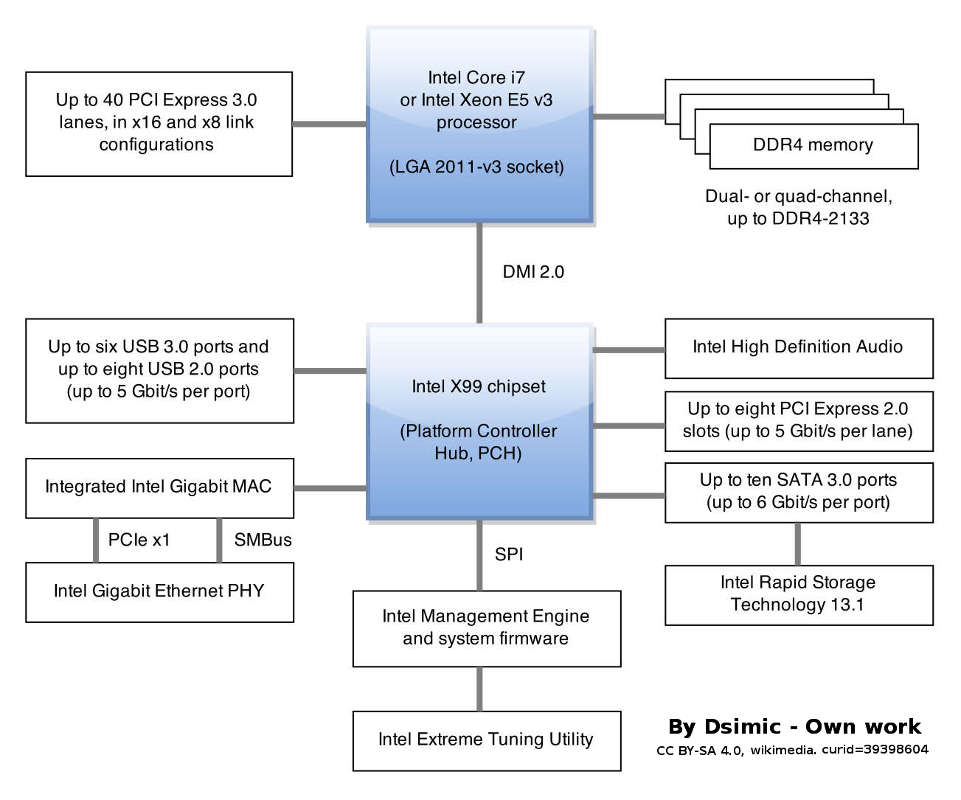
\includegraphics[width=0.53\linewidth]{os00-x99-chipset-block-diagram}
\caption{PCH: Platform Controller Hub}
\end{figure}
\end{frame}

% XXXXXXXXXXXXXXXXXXXXXXXXXXXXXXXXXXXXXXXXXXXXXXXXXXXXXXXXXXXXXXXXXXXXXXXXXX
\begin{frame}
\frametitle{Some Terms}
\begin{itemize}
\item PCH: Platform Controller Hub
\begin{itemize}
\item The successor of north/south-bridge architecture chipsets.
\end{itemize}
\item PCIe: Peripheral Component Interconnect Express
\begin{itemize}
\item 1 lane = dual simplex channel (1x); 2 lanes = 2x; etc.
\item 40 lanes = 8 GTs (GigaTransfers per second).
\item Configurations: 8x and 16x.
\end{itemize}
\item DDR4 SDRAM (single/dual/quad channel(s))
\begin{itemize}
\item Double Data Rate Fourth-generation Synchronous Dynamic Random-Access Memory:
      2 x DDR2 (DDR2 = 2 x DDR (DDR = 2 x SDRAM)).
      Eg. DDR4-3200 (8x SDRAM); Memory Clock: 400 MHz; Data Rate: 3200 MT/s; Module Name PC4-25600;
      Peak Transfer Rate: 25600 MB/s,
\end{itemize}
\item DMI 2.0 (Direct Media Interface): 4x.
\item SMB: System Management Bus
\item SPI: Serial Peripheral Interface, a de facto standard bus.
\item SATA:  Serial AT Attachment. Eg. SATA 3.2 $\approx$ 2 GB/s.
\item 1 KB (KiloByte) = 1000 bytes --- 1 KiB (Kibibyte) = 1024 bytes\footnote{%
      In IT tradition; 1 KB = 1024 bytes}
\end{itemize}
\end{frame}

% XXXXXXXXXXXXXXXXXXXXXXXXXXXXXXXXXXXXXXXXXXXXXXXXXXXXXXXXXXXXXXXXXXXXXXXXXX
\section{Sockets}
\begin{frame}
\frametitle{Sockets}
\begin{itemize}
\item Sockets
\begin{itemize}
\item \texttt{atoi()}
\item \texttt{accept()}
\item \texttt{bind()}
\item \texttt{connect()}
\item \texttt{exit()}
\item \texttt{fprintf()}
\item \texttt{getenv()}
\item \texttt{gethostbyname()}
\item \texttt{htons()}
\item \texttt{listen()}
\item \texttt{memcpy()}
\item \texttt{memset()}
\end{itemize}
\end{itemize}
\end{frame}

% XXXXXXXXXXXXXXXXXXXXXXXXXXXXXXXXXXXXXXXXXXXXXXXXXXXXXXXXXXXXXXXXXXXXXXXXXX
\begin{frame}
\frametitle{Sockets}
\begin{itemize}
\item Sockets
\begin{itemize}
\item \texttt{perror()}
\item \texttt{sizeof()}
\item \texttt{socket()}
\item \texttt{snprintf()}
\item \texttt{strchr()}
\item \texttt{strcmp()}
\item \texttt{strncpy()}
\item \texttt{strlen()}
\item \texttt{read()}
\item \texttt{write()}
\end{itemize}
\end{itemize}
\end{frame}

% XXXXXXXXXXXXXXXXXXXXXXXXXXXXXXXXXXXXXXXXXXXXXXXXXXXXXXXXXXXXXXXXXXXXXXXXXX
\section{10-server}
\begin{frame}[fragile]
\frametitle{10-server (01)}
% \large(54) \small(65) \footnotesize(72) \tiny(108) 
% \begin{lstlisting}[basicstyle=\ttfamily\large]
% \begin{lstlisting}[basicstyle=\ttfamily\small]
\begin{lstlisting}[basicstyle=\ttfamily\footnotesize]
/* Copyright (C) 2007-2020 Rahmat M. Samik-Ibrahim
 * http://rahmatm.samik-ibrahim.vlsm.org/
 * This program is free script/software.
 * REV02 Sun May  3 07:53:26 WIB 2020
 * START Xxx Xxx XX XX:XX:XX UTC 2007
 */
char pesan[]="[FROM SERVER] ACK MESSAGE...\n";
#include <stdio.h>
#include <string.h>
#include <stdlib.h>
#include <unistd.h>
#include <netdb.h>
#include <sys/socket.h>
#include <arpa/inet.h>
typedef struct sockaddr    sockad;
typedef struct sockaddr_in sockadin;
typedef struct hostent     shostent;

\end{lstlisting}
\end{frame}

% XXXXXXXXXXXXXXXXXXXXXXXXXXXXXXXXXXXXXXXXXXXXXXXXXXXXXXXXXXXXXXXXXXXXXXXXXX
\begin{frame}[fragile]
\frametitle{10-server (02)}
% \large(54) \small(65) \footnotesize(72) \tiny(108) 
% \begin{lstlisting}[basicstyle=\ttfamily\large]
% \begin{lstlisting}[basicstyle=\ttfamily\small]
% \begin{lstlisting}[basicstyle=\ttfamily\footnotesize]
\begin{lstlisting}[basicstyle=\ttfamily\tiny]
void error(char *msg){
   perror(msg);
   exit(0);
}

int main(int argc, char *argv[]) {
   char     buffer[256];
   int      clilen, newsockfd, nn, portno, sockfd;
   sockadin serv_addr, cli_addr;

   if (argc < 2) {
      fprintf(stderr, "ERROR, no port provided\n");
      exit(1);
   }
   sockfd = socket(AF_INET, SOCK_STREAM, 0);
   if (sockfd < 0)
      error("ERROR opening socket");
   int enable = 1;
   if (setsockopt(sockfd, SOL_SOCKET, SO_REUSEADDR, 
       &enable, sizeof(int)) < 0)
      error("setsockopt(SO_REUSEADDR) failed");
   memset(&serv_addr, 0, sizeof(serv_addr));
   portno = atoi(argv[1]);
   serv_addr.sin_family      = AF_INET;
   serv_addr.sin_addr.s_addr = INADDR_ANY;
   serv_addr.sin_port        = htons(portno);
   if (bind(sockfd, (sockad*) &serv_addr, sizeof(serv_addr))< 0)
      error("ERROR on binding");
   listen(sockfd, 5);
   clilen = sizeof(cli_addr);

\end{lstlisting}
\end{frame}

% XXXXXXXXXXXXXXXXXXXXXXXXXXXXXXXXXXXXXXXXXXXXXXXXXXXXXXXXXXXXXXXXXXXXXXXXXX
\begin{frame}[fragile]
\frametitle{10-server (03)}
% \large(54) \small(65) \footnotesize(72) \tiny(108) 
% \begin{lstlisting}[basicstyle=\ttfamily\large]
% \begin{lstlisting}[basicstyle=\ttfamily\small]
% \begin{lstlisting}[basicstyle=\ttfamily\tiny]
\begin{lstlisting}[basicstyle=\ttfamily\footnotesize]
   newsockfd=accept(sockfd,(sockad*)&cli_addr,
      (socklen_t*)&clilen);
   if (newsockfd < 0) error("ERROR on accept");
   memset(buffer, 0, 256);
   nn = read(newsockfd,buffer,255);
   if (nn < 0) error("ERROR reading from socket");
   printf("[FROM CLIENT]:\n %s\n",buffer);
   nn = write(newsockfd, pesan, sizeof(pesan));
   if (nn < 0) error("ERROR writing to socket");
   return 0;
}

\end{lstlisting}
\end{frame}

% XXXXXXXXXXXXXXXXXXXXXXXXXXXXXXXXXXXXXXXXXXXXXXXXXXXXXXXXXXXXXXXXXXXXXXXXXX
\section{11-client}
\begin{frame}[fragile]
\frametitle{11-client (01)}
% \large(54) \small(65) \footnotesize(72) \tiny(108) 
% \begin{lstlisting}[basicstyle=\ttfamily\large]
% \begin{lstlisting}[basicstyle=\ttfamily\footnotesize]
% \begin{lstlisting}[basicstyle=\ttfamily\tiny]
\begin{lstlisting}[basicstyle=\ttfamily\small]
/* Copyright (C) 2007-2018 Rahmat M. Samik-Ibrahim
 * http://rahmatm.samik-ibrahim.vlsm.org/
 * This program is free script/software.
 * REV01 Wed Aug 29 20:53:11 WIB 2018
 * START Xxx Xxx XX XX:XX:XX UTC 2007
 */
char pesan[]="[FROM SERVER] ACK MESSAGE...\n";
#include <stdio.h>
#include <string.h>
#include <stdlib.h>
#include <unistd.h>
#include <netdb.h>
#include <sys/socket.h>
#include <arpa/inet.h>
typedef struct sockaddr    sockad;
typedef struct sockaddr_in sockadin;
typedef struct hostent     shostent;

\end{lstlisting}
\end{frame}

% XXXXXXXXXXXXXXXXXXXXXXXXXXXXXXXXXXXXXXXXXXXXXXXXXXXXXXXXXXXXXXXXXXXXXXXXXX
\begin{frame}[fragile]
\frametitle{11-client (02)}
% \large(54) \small(65) \footnotesize(72) \tiny(108) 
% \begin{lstlisting}[basicstyle=\ttfamily\large]
% \begin{lstlisting}[basicstyle=\ttfamily\small]
% \begin{lstlisting}[basicstyle=\ttfamily\footnotesize]
\begin{lstlisting}[basicstyle=\ttfamily\tiny]
void error(char *msg){
   perror(msg);
   exit(0);
}

int main(int argc, char *argv[]) {
   char      buffer[256];
   int       nn, portno, sockfd;
   sockadin  serv_addr;
   shostent* server;
   if (argc < 3) {
      fprintf(stderr, "usage %s hostname port\n", argv[0]);
      exit(0);
   }
   portno = atoi(argv[2]);
   sockfd = socket(AF_INET,SOCK_STREAM,0);
   if (sockfd < 0)
      error("ERROR opening socket");
   server = gethostbyname(argv[1]);
   if (server == NULL) {
     fprintf(stderr, "ERROR, no such host\n");
     exit(0);
   }
   memset(&serv_addr,0,sizeof(serv_addr));
   serv_addr.sin_family = AF_INET;
   memmove( &serv_addr.sin_addr.s_addr, server->h_addr, server->h_length);
   serv_addr.sin_port   = htons(portno);
   if(connect(sockfd,(const struct sockaddr*) &serv_addr, sizeof(serv_addr))<0)
       error("ERROR connecting");
   printf("Enter the message: ");
   memset(buffer,   0, 256);

\end{lstlisting}
\end{frame}

% XXXXXXXXXXXXXXXXXXXXXXXXXXXXXXXXXXXXXXXXXXXXXXXXXXXXXXXXXXXXXXXXXXXXXXXXXX
\begin{frame}[fragile]
\frametitle{11-client (03)}
% \large(54) \small(65) \footnotesize(72) \tiny(108) 
% \begin{lstlisting}[basicstyle=\ttfamily\large]
% \begin{lstlisting}[basicstyle=\ttfamily\small]
% \begin{lstlisting}[basicstyle=\ttfamily\footnotesize]
\begin{lstlisting}[basicstyle=\ttfamily\tiny]
   fgets (buffer, 255, stdin);
   nn = write(sockfd,buffer,strlen(buffer));
   if (nn < 0)
      error("ERROR writing to socket");
   memset(buffer, 0, 256);
   nn = read(sockfd,buffer,255);
   if (nn < 0)
      error("ERROR reading from socket");
   printf("%s\n",buffer);
   return 0;
}

# TERMINAL 1 #########################################

$ ./10-server 6666
[FROM CLIENT]:
 Hello World!
$


# TERMINAL 2 #########################################

$ ./11-client localhost 6666
Enter the message: Hello World!
[FROM SERVER] ACK MESSAGE...

$

\end{lstlisting}
\end{frame}

% XXXXXXXXXXXXXXXXXXXXXXXXXXXXXXXXXXXXXXXXXXXXXXXXXXXXXXXXXXXXXXXXXXXXXXXXXX
\section{12-clisvr}
\begin{frame}[fragile]
\frametitle{12-clisvr (01)}
% \large(54) \small(65) \footnotesize(72) \tiny(108) 
% \begin{lstlisting}[basicstyle=\ttfamily\large]
% \begin{lstlisting}[basicstyle=\ttfamily\small]
% \begin{lstlisting}[basicstyle=\ttfamily\footnotesize]
\begin{lstlisting}[basicstyle=\ttfamily\tiny]
/*
 * Copyright (C) 2007 Tadeus Prastowo
 * Copyright (C) 2017 - 2020 Rahmat M. Samik-Ibrahim
 * http://rahmatm.samik-ibrahim.vlsm.org/
 * This program is free script/software. This program is distributed in the 
 * hope that it will be useful, but WITHOUT ANY WARRANTY; without even the 
 * implied warranty of MERCHANTABILITY or FITNESS FOR A PARTICULAR PURPOSE.
 * REV04 Sun May  3 07:59:57 WIB 2020
 * REV03 Wed Feb 27 19:21:44 WIB 2019
 * REV02 Wed Aug 29 20:54:25 WIB 2018
 * REV01 Wed Nov  8 20:00:02 WIB 2017
 * START 2007
 *
 * This program serves as both a client and a server. Three modes of
 * operation are available:
 *  - initiating mode
 *  - bridging mode
 *  - terminating mode
 *
 * The following are how to run thisprogram for each mode:
 *  - Initiating mode:  client_server null ANOTHER_HOST ANOTHER_PORT
 *  - Bridging mode:    client_server CURRENT_PORT ANOTHER_HOST ANOTHER_PORT
 *  - Terminating mode: client_server CURRENT_PORT null null
 *
 * The program having the initiating mode _MUST_ run last after all other
 * instances of this program with other operational modes has been started.
 *
 * In initiating mode, this program just simply sends a hello message to
 * another instance of this program that operates either as a bridge or
 * as a terminator that this program points to as specified in
 * ANOTHER_HOST and ANOTHER_PORT. After that this program will quit
 * without printing out any message.
 *
 * In bridging mode, this program just simply waits for an incoming hello
 * message in CURRENT_PORT. Once it receives a hello message, it prints
 * out the message in a certain format. Next, this program forwards the
 * modified message to another instance of this program that acts either as
 * a bridge or as a terminator that this program points to as specified
 * in ANOTHER_HOST and ANOTHER_PORT. After that this program will quit.
 *

\end{lstlisting}
\end{frame}

% XXXXXXXXXXXXXXXXXXXXXXXXXXXXXXXXXXXXXXXXXXXXXXXXXXXXXXXXXXXXXXXXXXXXXXXXXX
\begin{frame}[fragile]
\frametitle{12-clisvr (02)}
% \large(54) \small(65) \footnotesize(72) \tiny(108) 
% \begin{lstlisting}[basicstyle=\ttfamily\large]
% \begin{lstlisting}[basicstyle=\ttfamily\small]
% \begin{lstlisting}[basicstyle=\ttfamily\footnotesize]
\begin{lstlisting}[basicstyle=\ttfamily\tiny]
 * In terminating mode, this program just simply waits for an incoming hello
 * message in CURRENT_PORT. Once it receives a hello message, it prints out
 * the message in a certain format, and then quits.
 *
 * The following illustrates the idea above:
 * 192.168.10.18 (alvin)
 * $ ./client_server 8888 localhost 7777
 * 192.168.10.18 (user)$
 * $ ./client_server 7777 null null
 * 192.168.12.17 (eus)$
 * $ ./client_server null 192.168.10.18 8888
 * The print out will be:
 * 192.168.10.18 (alvin):
 *   From eus to alvin: Hello
 * 192.168.10.18 (user):
 *   From eus to alvin to user: Hello
 */

char pesan[]="[FROM SERVER] ACK MESSAGE...\n";

#include <stdio.h>
#include <string.h>
#include <stdlib.h>
#include <unistd.h>
#include <netdb.h>
#include <sys/time.h>
#include <sys/socket.h>
#include <arpa/inet.h>

typedef struct sockaddr    sockad;
typedef struct sockaddr_in sockadin;
typedef struct hostent     shostent;

\end{lstlisting}
\end{frame}

% XXXXXXXXXXXXXXXXXXXXXXXXXXXXXXXXXXXXXXXXXXXXXXXXXXXXXXXXXXXXXXXXXXXXXXXXXX
\begin{frame}[fragile]
\frametitle{12-clisvr (03)}
% \large(54) \small(65) \footnotesize(72) \tiny(108) 
% \begin{lstlisting}[basicstyle=\ttfamily\large]
% \begin{lstlisting}[basicstyle=\ttfamily\small]
% \begin{lstlisting}[basicstyle=\ttfamily\footnotesize]
\begin{lstlisting}[basicstyle=\ttfamily\tiny]

void error(char *msg){
   perror(msg);
   exit(0);
}

#define BUFFER_SIZE 4096

int main(int argc, char *argv []) {
   int sockfd, newsockfd, portno, clilen, count, nn, sysup;
   char buffer [BUFFER_SIZE], temp_buffer [BUFFER_SIZE], *colon_pos;
   struct sockaddr_in serv_addr, cli_addr;
   struct hostent *server;
   struct timeval tval;

   if (argc < 4) {
      fprintf (stderr,"\nUsage: %s this_port  next_sever next_server_port\n\n"
               "Start the chain with `this_port' = `null'\n\n"
               "Terminte the chain with `next_server' = `next_server_port'"
               " = `null'\n\n", argv [0]);
      exit (1);
   }
   if (strcmp (argv [1], "null") == 0) {
      portno = atoi   (argv [3]);
      sockfd = socket (AF_INET, SOCK_STREAM, 0);
      if (sockfd < 0) {
         error ("ERROR opening socket");
      }
      int enable = 1;
      if (setsockopt(sockfd, SOL_SOCKET, SO_REUSEADDR, 
         &enable, sizeof(int)) < 0)
         error("setsockopt(SO_REUSEADDR) failed");

\end{lstlisting}
\end{frame}

% XXXXXXXXXXXXXXXXXXXXXXXXXXXXXXXXXXXXXXXXXXXXXXXXXXXXXXXXXXXXXXXXXXXXXXXXXX
\begin{frame}[fragile]
\frametitle{12-clisvr (04)}
% \large(54) \small(65) \footnotesize(72) \tiny(108) 
% \begin{lstlisting}[basicstyle=\ttfamily\large]
% \begin{lstlisting}[basicstyle=\ttfamily\small]
% \begin{lstlisting}[basicstyle=\ttfamily\footnotesize]
\begin{lstlisting}[basicstyle=\ttfamily\tiny]
      server = gethostbyname(argv[2]);
      if (server == NULL) {
         fprintf (stderr, "ERROR, no such host\n");
         exit (1);
      }
      memset (&serv_addr, 0, sizeof (serv_addr));
      serv_addr.sin_family = AF_INET;
      memcpy(&serv_addr.sin_addr.s_addr, server->h_addr, server->h_length);
      serv_addr.sin_port = htons(portno);
      if (connect(sockfd,(struct sockaddr *)&serv_addr,sizeof(serv_addr))< 0){
         error ("ERROR connecting");
      }
      /* Begin: action */
      memset (buffer, 0, BUFFER_SIZE);
      gettimeofday(&tval,NULL);
      sysup = 0x0000FFFF & (int) (tval.tv_sec * 1000 + tval.tv_usec / 1000);
      snprintf (buffer, BUFFER_SIZE, "From\n%s[%d]:", getenv ("USER"), sysup);
      nn = write (sockfd, buffer, strlen (buffer));
      if (nn < 0) {
        error ("ERROR writing to socket");
      }
      /* End: action */
      exit (0);
   }

   sockfd = socket(AF_INET,SOCK_STREAM,0);
   if (sockfd < 0) {
      error ("ERROR opening socket");
   }

\end{lstlisting}
\end{frame}

% XXXXXXXXXXXXXXXXXXXXXXXXXXXXXXXXXXXXXXXXXXXXXXXXXXXXXXXXXXXXXXXXXXXXXXXXXX
\begin{frame}[fragile]
\frametitle{12-clisvr (05)}
% \large(54) \small(65) \footnotesize(72) \tiny(108) 
% \begin{lstlisting}[basicstyle=\ttfamily\large]
% \begin{lstlisting}[basicstyle=\ttfamily\small]
% \begin{lstlisting}[basicstyle=\ttfamily\footnotesize]
\begin{lstlisting}[basicstyle=\ttfamily\tiny]
   int enable = 1;
   if (setsockopt(sockfd, SOL_SOCKET, SO_REUSEADDR, 
      &enable, sizeof(int)) < 0)
      error("setsockopt(SO_REUSEADDR) failed");
   memset(&serv_addr,0,sizeof(serv_addr));
   portno = atoi (argv [1]);
   serv_addr.sin_family = AF_INET;
   serv_addr.sin_addr.s_addr = INADDR_ANY;
   serv_addr.sin_port = htons (portno);
   if (bind (sockfd,(struct sockaddr *)&serv_addr, sizeof(serv_addr)) < 0) {
      error ("ERROR on binding");
   }
   listen (sockfd, 5);
   clilen    = sizeof (cli_addr);
   newsockfd = accept (sockfd, (struct sockaddr *) &cli_addr,
               (socklen_t *) &clilen);
   if (newsockfd < 0) {
      error ("ERROR on accept");
   }
   memset (buffer, 0, BUFFER_SIZE);
   nn = read(newsockfd,buffer,BUFFER_SIZE-1);
   if (nn < 0) {
      error ("ERROR reading from socket");
   }
   /* Modify buffer's message */
   colon_pos = strchr (buffer, ':');
   nn        = colon_pos - buffer;
   memset (temp_buffer, 0, BUFFER_SIZE);
   strncpy (temp_buffer, buffer, nn);
   memset (buffer, 0, BUFFER_SIZE);
   strncpy (buffer, temp_buffer, nn);

\end{lstlisting}
\end{frame}

% XXXXXXXXXXXXXXXXXXXXXXXXXXXXXXXXXXXXXXXXXXXXXXXXXXXXXXXXXXXXXXXXXXXXXXXXXX
\begin{frame}[fragile]
\frametitle{12-clisvr (06)}
% \large(54) \small(65) \footnotesize(72) \tiny(108) 
% \begin{lstlisting}[basicstyle=\ttfamily\large]
% \begin{lstlisting}[basicstyle=\ttfamily\small]
% \begin{lstlisting}[basicstyle=\ttfamily\footnotesize]
\begin{lstlisting}[basicstyle=\ttfamily\tiny]
   for (long ii=0; ii<5000000L; ii++)
      ; // delay
   gettimeofday(&tval,NULL);
   sysup = 0x0000FFFF & (int) (tval.tv_sec * 1000 + tval.tv_usec / 1000);
   snprintf (buffer + nn, BUFFER_SIZE-nn, " to\n%s[%d]:\nEndOfMessage!", getenv ("USER"), sysup);
   /*End of modifying buffer's message*/
   if (strcmp (argv [2], "null") != 0 && strcmp (argv [3], "null") != 0) {
      portno = atoi (argv [3]);
      sockfd=socket(AF_INET,SOCK_STREAM,0);
      if (sockfd < 0) {
         error ("ERROR opening socket");
      }
      server = gethostbyname (argv [2]);
      if (server == NULL) {
         fprintf (stderr, "ERROR, no such host\n");
         exit (1);
      }
      serv_addr.sin_family = AF_INET;
      memcpy (&serv_addr.sin_addr.s_addr, server->h_addr, server->h_length);
      serv_addr.sin_port = htons (portno);
      if (connect (sockfd,(struct sockaddr *)&serv_addr,sizeof (serv_addr))<0){
         error ("ERROR connecting");
      }
      printf ("%s\n", buffer); // ============ Begin: action
      nn=write(sockfd,buffer,strlen(buffer));
      if (nn < 0) error ("ERROR writing to socket"); // ============ End: action
      else printf ("%s\n", buffer);
   return 0;
}

\end{lstlisting}
\end{frame}

% XXXXXXXXXXXXXXXXXXXXXXXXXXXXXXXXXXXXXXXXXXXXXXXXXXXXXXXXXXXXXXXXXXXXXXXXXX
\begin{frame}[fragile]
\frametitle{12-clisvr (07)}

\begin{figure}
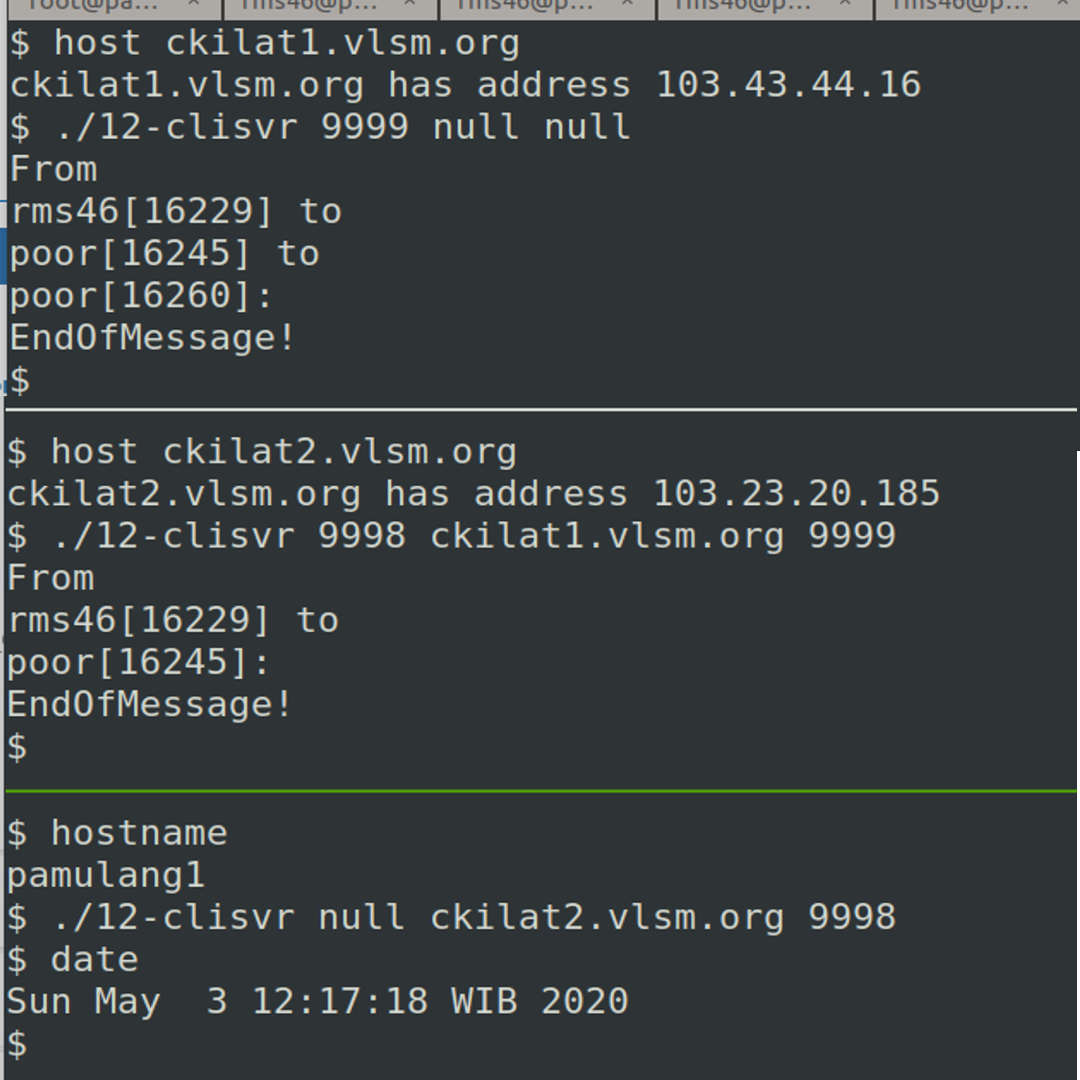
\includegraphics[width=0.43\linewidth]{os-clisvr}
\caption{Client Server}
\end{figure}

\end{frame}

% XXXXXXXXXXXXXXXXXXXXXXXXXXXXXXXXXXXXXXXXXXXXXXXXXXXXXXXXXXXXXXXXXXXXXXXXXX
\section{54-write}
\begin{frame}[fragile]
\frametitle{54-write (01)}
% \large(54) \small(65) \footnotesize(72) \tiny(108) 
% \begin{lstlisting}[basicstyle=\ttfamily\large]
% \begin{lstlisting}[basicstyle=\ttfamily\small]
% \begin{lstlisting}[basicstyle=\ttfamily\footnotesize]
\begin{lstlisting}[basicstyle=\ttfamily\tiny]
/*
 * Copyright (C) 2015-2019 Rahmat M. Samik-Ibrahim
 * http://rahmatm.samik-ibrahim.vlsm.org/
 * This program is free script/software. This program is distributed in the 
 * hope that it will be useful, but WITHOUT ANY WARRANTY; without even the 
 * implied warranty of MERCHANTABILITY or FITNESS FOR A PARTICULAR PURPOSE.
 *
 * TAKE NOTE()
 * O_RDWR open for reading and writing
 * O_CREAT indicates that the call to open() has a mode argument,
 * if the file being opened already exist O_CREAT has no effect
 * if the file being opened does not exist it is created
 * if O_CREAT is specified and the file did not previously exist a sucessful open
 * () sets the access time, change time, and modification time for the file
 *
 * if succesful, dup() returns a new file descriptor
 * if unsucessful, dup() returs -1 and sets errno to EBADF or EMFILE
 *
 * REV09 Tue Nov 26 11:38:34 WIB 2019
 * REV08 Wed Aug 29 20:55:23 WIB 2018
 * REV07 Thu Oct  5 17:56:09 WIB 2017
 * REV02 Sun Oct 16 20:50:52 WIB 2016
 * START Xxx Apr 25 XX:XX:XX WIB 2015
 */

#include <stdio.h>
#include <sys/types.h>
#include <sys/stat.h>
#include <fcntl.h>
#include <unistd.h>
#include <string.h>

\end{lstlisting}
\end{frame}

% 14
% XXXXXXXXXXXXXXXXXXXXXXXXXXXXXXXXXXXXXXXXXXXXXXXXXXXXXXXXXXXXXXXXXXXXXXXXXX
\begin{frame}[fragile]
\frametitle{54-write (02)}
% \large(54) \small(65) \footnotesize(72) \tiny(108) 
% \begin{lstlisting}[basicstyle=\ttfamily\large]
% \begin{lstlisting}[basicstyle=\ttfamily\small]
% \begin{lstlisting}[basicstyle=\ttfamily\footnotesize]
\begin{lstlisting}[basicstyle=\ttfamily\tiny]
#define  FILE5   "demo-file5.txt"
static char* str1 = "AAAXBBB\n";
static char* str2 = "CCC\n";

void main(void) {
   int fd1, fd2;
   fd1 = open (FILE5, O_RDWR | O_CREAT, 0644);
   fd2 = open (FILE5, O_RDWR | O_CREAT, 0644);
   printf("File Descriptors --- fd1 = %d, fd2 = %d\n", fd1, fd2);
   write(fd1, str1, strlen(str1));
   write(fd2, str2, strlen(str2));
   close(fd1);
   close(fd2);
   printf("See output file %s\n", FILE5);
}
# #####################################
$ ./54-write 
File Descriptors --- fd1 = 3, fd2 = 4
See output file demo-file5.txt

$ cat demo-file5.txt 
CCC
BBB

$ 

\end{lstlisting}
\end{frame}

% XXXXXXXXXXXXXXXXXXXXXXXXXXXXXXXXXXXXXXXXXXXXXXXXXXXXXXXXXXXXXXXXXXXXXXXXXX
\section{55-write}
\begin{frame}[fragile]
\frametitle{55-write (01)}
% \large(54) \small(65) \footnotesize(72) \tiny(108) 
% \begin{lstlisting}[basicstyle=\ttfamily\large]
% \begin{lstlisting}[basicstyle=\ttfamily\small]
% \begin{lstlisting}[basicstyle=\ttfamily\footnotesize]
\begin{lstlisting}[basicstyle=\ttfamily\tiny]
/*
 * Copyright (C) 2015-2019 Rahmat M. Samik-Ibrahim
 * http://rahmatm.samik-ibrahim.vlsm.org/
 * This program is free script/software. This program is distributed in the 
 * hope that it will be useful, but WITHOUT ANY WARRANTY; without even the 
 * implied warranty of MERCHANTABILITY or FITNESS FOR A PARTICULAR PURPOSE.
 *
 * TAKE NOTE (MA)
 * Program ini akan membuat file baru dengan isi
 * buf1 pada 8 char pertama, dan buf2 pada 8 char terakhir
 *
 * Line 31 akan membuat program menulis 8 char 
 * dari variabel char buf1 ke file yang didefine pada Line 19
 *
 * Line 35 akan membuat offset menjadi 32,
 * yang maksudnya adalah pointernya lompat ke huruf ke 32
 * Sehingga ketika menulis lg, akan dimulai pada huruf ke 33
 *
 * REV06 Tue Nov 26 11:39:10 WIB 2019
 * REV05 Wed Aug 29 20:55:23 WIB 2018
 * REV04 Wed Oct 18 17:54:25 WIB 2017
 * REV02 Thu Mar  9 21:21:28 WIB 2017
 * START Xxx Apr 25 XX:XX:XX WIB 2015
 * USE "hexdump FILE1"
 */

#include <stdio.h>
#include <stdlib.h>
#include <unistd.h>
#include <sys/types.h>
#include <sys/stat.h>
#include <fcntl.h>

\end{lstlisting}
\end{frame}

% XXXXXXXXXXXXXXXXXXXXXXXXXXXXXXXXXXXXXXXXXXXXXXXXXXXXXXXXXXXXXXXXXXXXXXXXXX
\begin{frame}[fragile]
\frametitle{54-write (02)}
% \large(54) \small(65) \footnotesize(72) \tiny(108) 
% \begin{lstlisting}[basicstyle=\ttfamily\large]
% \begin{lstlisting}[basicstyle=\ttfamily\small]
% \begin{lstlisting}[basicstyle=\ttfamily\footnotesize]
\begin{lstlisting}[basicstyle=\ttfamily\tiny]
#define  FILE6   "demo-file6.txt"
char buf1[] = "abcdefgh";
char buf2[] = "ABCDEFGH";
void main(void) {
   int fd;
   fd = creat(FILE6, 0644);
   if (fd < 0) {
      perror("creat error");
      exit(1);
   }
   if (write(fd, buf1, 8) != 8) {
      perror("buf1 write error");
      exit(1);
   } /* offset now = 8 */
   if (lseek(fd, 32, SEEK_SET) == -1) {
      perror("lseek error");
      exit(1);
   } /* offset now = 32 */
   if (write(fd, buf2, 8) != 8) {
      perror("buf2 write error");
      exit(1);
   } /* offset now = 40 */
   close(fd);
   printf("Run: hexdump -c %s\n", FILE6);
}
# ###
$ hexdump -c demo-file6.txt 
0000000   a   b   c   d   e   f   g   h  \0  \0  \0  \0  \0  \0  \0  \0
0000010  \0  \0  \0  \0  \0  \0  \0  \0  \0  \0  \0  \0  \0  \0  \0  \0
0000020   A   B   C   D   E   F   G   H                                
0000028
\end{lstlisting}
\end{frame}

% XXXXXXXXXXXXXXXXXXXXXXXXXXXXXXXXXXXXXXXXXXXXXXXXXXXXXXXXXXXXXXXXXXXXXXXXXX
\section{57-dup}
\begin{frame}[fragile]
\frametitle{57-dup (01)}
% \large(54) \small(65) \footnotesize(72) \tiny(108) 
% \begin{lstlisting}[basicstyle=\ttfamily\large]
% \begin{lstlisting}[basicstyle=\ttfamily\small]
% \begin{lstlisting}[basicstyle=\ttfamily\footnotesize]
\begin{lstlisting}[basicstyle=\ttfamily\tiny]
/*
 * Copyright (C) 2016-2019 Rahmat M. Samik-Ibrahim
 * http://rahmatm.samik-ibrahim.vlsm.org/
 * This program is free script/software. This program is distributed in the 
 * hope that it will be useful, but WITHOUT ANY WARRANTY; without even the 
 * implied warranty of MERCHANTABILITY or FITNESS FOR A PARTICULAR PURPOSE.
 *
 * TAKE NOTE(TA)
 * O_RDWR open for reading and writing
 * O_CREAT indicates that the call to open() has a mode argument,
 * if the file being opened already exist O_CREAT has no effect
 * if the file being opened does not exist it is created
 * if O_CREAT is specified and the file did not previously exist a sucessful open
 * () sets the access time, change time, and modification time for the file
 *
 * if succesful, dup() returns a new file descriptor
 * if unsucessful, dup() returs -1 and sets errno to EBADF or EMFILE
 * 
 * REV07 Tue Nov 26 11:39:10 WIB 2019
 * START Xxx Apr 25 XX:XX:XX WIB 2015
 * dup(fd) duplicates fd
 * fd2=dup(fd1)  <---> dup2(fd1, fd2)
 */

#include <stdio.h>
#include <sys/types.h>
#include <sys/stat.h>
#include <fcntl.h>
#include <unistd.h>
#include <string.h>

\end{lstlisting}
\end{frame}

% XXXXXXXXXXXXXXXXXXXXXXXXXXXXXXXXXXXXXXXXXXXXXXXXXXXXXXXXXXXXXXXXXXXXXXXXXX
\begin{frame}[fragile]
\frametitle{57-dup (02)}
% \large(54) \small(65) \footnotesize(72) \tiny(108) 
% \begin{lstlisting}[basicstyle=\ttfamily\large]
% \begin{lstlisting}[basicstyle=\ttfamily\small]
% \begin{lstlisting}[basicstyle=\ttfamily\footnotesize]
\begin{lstlisting}[basicstyle=\ttfamily\tiny]
#define FILE1 "demo-file7.txt"
static char* str1 = "AAAXBBB\n";
static char* str2 = "CCC\n";
void main(void) {
   int fd1, fd2;
   fd1 = open (FILE1, O_RDWR | O_CREAT, 0644);
   fd2 = dup(fd1);
   printf("File Descriptors --- fd1 = %d, fd2 = %d\n", fd1, fd2);
   write(fd1, str1, strlen(str1));
   write(fd2, str2, strlen(str2));
   close(fd1);
   close(fd2);
   printf("**** Please check file %s *****\n", FILE1);
   printf("**** Compare with 54-write\n");
}
# #####
$ ./54-write 
File Descriptors --- fd1 = 3, fd2 = 4
See output file demo-file5.txt
$ ./57-dup 
File Descriptors --- fd1 = 3, fd2 = 4
**** Please check file demo-file7.txt *****
**** Compare with 54-write
$ cat demo-file5.txt 
CCC
BBB
$ cat demo-file7.txt 
AAAXBBB
CCC
$ 

\end{lstlisting}
\end{frame}

% XXXXXXXXXXXXXXXXXXXXXXXXXXXXXXXXXXXXXXXXXXXXXXXXXXXXXXXXXXXXXXXXXXXXXXXXXX
\section{58-dup2}
\begin{frame}[fragile]
\frametitle{58-dup2 (01)}
% \large(54) \small(65) \footnotesize(72) \tiny(108) 
% \begin{lstlisting}[basicstyle=\ttfamily\large]
% \begin{lstlisting}[basicstyle=\ttfamily\small]
% \begin{lstlisting}[basicstyle=\ttfamily\tiny]
\begin{lstlisting}[basicstyle=\ttfamily\footnotesize]
/*
 * Copyright (C) 2015-2019 Rahmat M. Samik-Ibrahim
 * http://rahmatm.samik-ibrahim.vlsm.org/
 * This program is free script/software. 
 * REV07 Tue May  7 18:46:12 WIB 2019
 * REV04 Thu Mar  9 21:22:36 WIB 2017
 * REV02 Sun Oct 16 20:52:15 WIB 2016
 * START Xxx Apr 25 XX:XX:XX WIB 2015
 *
 * fd2=dup2(fd1, NEWFD)
 *
 */

#include <stdio.h>
#include <sys/types.h>
#include <sys/stat.h>
#include <fcntl.h>
#include <unistd.h>
#include <string.h>

\end{lstlisting}
\end{frame}

% XXXXXXXXXXXXXXXXXXXXXXXXXXXXXXXXXXXXXXXXXXXXXXXXXXXXXXXXXXXXXXXXXXXXXXXXXX
\begin{frame}[fragile]
\frametitle{58-dup2 (02)}
% \large(54) \small(65) \footnotesize(72) \tiny(108) 
% \begin{lstlisting}[basicstyle=\ttfamily\large]
% \begin{lstlisting}[basicstyle=\ttfamily\small]
% \begin{lstlisting}[basicstyle=\ttfamily\footnotesize]
\begin{lstlisting}[basicstyle=\ttfamily\tiny]
#define FILE1 "demo-file8.txt"
#define NEWFD 10
static char* str1 = "AAAXBBB\n";
static char* str2 = "CCC\n";
void main(void) {
   int fd1, fd2;
   fd1 = open (FILE1, O_RDWR | O_CREAT, 0644);
   fd2=dup2(fd1, NEWFD);
   printf("File Descriptors --- fd1 = %d, fd2 = %d\n", fd1, fd2);
   write(fd1, str1, strlen(str1));
   write(fd2, str2, strlen(str2));
   close(fd1);
   close(fd2);
   printf("**** Please check file %s *****\n", FILE1);
   printf("**** Compare with 54-write\n");
}

# ######

$ ./58-dup2 
File Descriptors --- fd1 = 3, fd2 = 10
**** Please check file demo-file8.txt *****
**** Compare with 54-write
$ cat demo-file8.txt 
AAAXBBB
CCC
$ cat demo-file5.txt 
CCC
BBB
$ 

\end{lstlisting}
\end{frame}

% XXXXXXXXXXXXXXXXXXXXXXXXXXXXXXXXXXXXXXXXXXXXXXXXXXXXXXXXXXXXXXXXXXXXXXXXXX
\section{59a-IO}
\begin{frame}[fragile]
\frametitle{59a-IO}
% \large(54) \small(65) \footnotesize(72) \tiny(108) 
% \begin{lstlisting}[basicstyle=\ttfamily\large]
% \begin{lstlisting}[basicstyle=\ttfamily\small]
% \begin{lstlisting}[basicstyle=\ttfamily\footnotesize]
\begin{lstlisting}[basicstyle=\ttfamily\tiny]
$ cat 59a-io.c 
// Copyright (C) 2015-2019 Rahmat M. Samik-Ibrahim
#define FILE1 "59a-io-demo.txt"
void main(void) {
   int fd1, fd2;
   char strvar[100];
   printf ("***** Please check file %s ***** *****\n", FILE1);
   fd1 = open (FILE1, O_RDWR | O_CREAT | O_TRUNC, 0644);
   fd2 = dup(fd1);
   printf(         "AAAAA print to standard output!!\n"); 
   fprintf(stdout, "BBBBB print to standard output!!\n"); 
   fprintf(stderr, "CCCCC print to standard error!!!\n");
   sprintf(strvar, "DDDDD print to fd1=%d!!!\n", fd1);
   dprintf(fd1,    "%s", strvar);
   dprintf(fd2,    "EEEEE print to fd2=%d!!!\n", fd2);
   close(fd1);
   close(fd2);
}
# ########
$ ./59a-io 
***** Please check file 59a-io-demo.txt ***** *****
AAAAA print to standard output!!
BBBBB print to standard output!!
CCCCC print to standard error!!!
$ cat 59a-io-demo.txt 
DDDDD print to fd1=3!!!
EEEEE print to fd2=4!!!
$ 

\end{lstlisting}
\end{frame}

% XXXXXXXXXXXXXXXXXXXXXXXXXXXXXXXXXXXXXXXXXXXXXXXXXXXXXXXXXXXXXXXXXXXXXXXXXX
\section{59b-IO}
\begin{frame}[fragile]
\frametitle{59b-IO}
% \large(54) \small(65) \footnotesize(72) \tiny(108) 
% \begin{lstlisting}[basicstyle=\ttfamily\large]
% \begin{lstlisting}[basicstyle=\ttfamily\small]
% \begin{lstlisting}[basicstyle=\ttfamily\footnotesize]
\begin{lstlisting}[basicstyle=\ttfamily\tiny]
// Copyright (C) 2015-2019 Rahmat M. Samik-Ibrahim
// #include ETC ETC
#define FILE1 "59b-io-demo.txt"
void main(void) {
   int fd1, fd2;
   char strvar[100];
   printf ("***** Please check file %s ***** *****\n", FILE1);
   close(STDERR_FILENO);
   fd1 = open (FILE1, O_RDWR | O_CREAT | O_TRUNC, 0644);
   fd2 = dup(fd1);
   printf(         "AAAAA print to standard output!!\n"); 
   fprintf(stdout, "BBBBB print to standard output!!\n"); 
   fprintf(stderr, "CCCCC print to standard error!!!\n");
   sprintf(strvar, "DDDDD print to fd1=%d!!!\n", fd1);
   dprintf(fd1,    "%s", strvar);
   dprintf(fd2,    "EEEEE print to fd2=%d!!!\n", fd2);
   close(fd1);
   close(fd2);
}
# ########
$ 
$ ./59b-io 
***** Please check file 59b-io-demo.txt ***** *****
AAAAA print to standard output!!
BBBBB print to standard output!!
$ cat 59b-io-demo.txt 
CCCCC print to standard error!!!
DDDDD print to fd1=2!!!
EEEEE print to fd2=3!!!
$ 

\end{lstlisting}
\end{frame}

% XXXXXXXXXXXXXXXXXXXXXXXXXXXXXXXXXXXXXXXXXXXXXXXXXXXXXXXXXXXXXXXXXXXXXXXXXX
\section{59c-IO}
\begin{frame}[fragile]
\frametitle{59c-IO}
% \large(54) \small(65) \footnotesize(72) \tiny(108) 
% \begin{lstlisting}[basicstyle=\ttfamily\large]
% \begin{lstlisting}[basicstyle=\ttfamily\small]
% \begin{lstlisting}[basicstyle=\ttfamily\footnotesize]
\begin{lstlisting}[basicstyle=\ttfamily\tiny]
// Copyright (C) 2015-2019 Rahmat M. Samik-Ibrahim
// #include ETC ETC
#define FILE1 "59c-io-demo.txt"

void main(void) {
   int fd1, fd2;
   char strvar[100];
   printf ("***** Please check file %s ***** *****\n", FILE1);
   close(STDERR_FILENO);
   close(STDOUT_FILENO);
   fd1 = open (FILE1, O_RDWR | O_CREAT | O_TRUNC, 0644);
   fd2 = dup(fd1);
   printf(         "AAAAA print to standard output!!\n"); 
   fprintf(stdout, "BBBBB print to standard output!!\n"); 
   fprintf(stderr, "CCCCC print to standard error!!!\n");
   sprintf(strvar, "DDDDD print to fd1=%d!!!\n", fd1);
   dprintf(fd1,    "%s", strvar);
   dprintf(fd2,    "EEEEE print to fd2=%d!!!\n", fd2);
   close(fd1);
   close(fd2);
}
# ######
$ ./59c-io 
***** Please check file 59c-io-demo.txt ***** *****
$ cat 59c-io-demo.txt 
AAAAA print to standard output!!
BBBBB print to standard output!!
CCCCC print to standard error!!!
DDDDD print to fd1=1!!!
EEEEE print to fd2=2!!!

\end{lstlisting}
\end{frame}

% XXXXXXXXXXXXXXXXXXXXXXXXXXXXXXXXXXXXXXXXXXXXXXXXXXXXXXXXXXXXXXXXXXXXXXXXXX
\begin{frame}[fragile]
\frametitle{70-os161}
% \large(54) \small(65) \footnotesize(72) \tiny(108) 
% \begin{lstlisting}[basicstyle=\ttfamily\large]
% \begin{lstlisting}[basicstyle=\ttfamily\small]
% \begin{lstlisting}[basicstyle=\ttfamily\footnotesize]
\begin{lstlisting}[basicstyle=\ttfamily\tiny]
// Copyright (C) 2015-2020 Rahmat M. Samik-Ibrahim
// #include ETC ETC

#include <stdio.h>
#include <string.h>
#include <unistd.h>
#include <fcntl.h>
#include <sys/types.h>
#include <sys/stat.h>

#define FILE "70-os161-demo.txt"

char *string = "ABCD\n";
void main(void) {
   int fileDescriptor;
   printf("See also file %s\n", FILE);
   close(STDOUT_FILENO);
   fileDescriptor = open (FILE, O_RDWR|O_CREAT|O_TRUNC, 0644);
   printf ( "%s", string);
   write(fileDescriptor, string, strlen(string));
}

# ######

$ ./70-os161 
See also file 70-os161-demo.txt

$ cat 70-os161-demo.txt 
ABCD
ABCD

\end{lstlisting}
\end{frame}

% XXXXXXXXXXXXXXXXXXXXXXXXXXXXXXXXXXXXXXXXXXXXXXXXXXXXXXXXXXXXXXXXXXXXXXXXXX
\section{71-os171}
\begin{frame}[fragile]
\frametitle{71-os171}
% \large(54) \small(65) \footnotesize(72) \tiny(108) 
% \begin{lstlisting}[basicstyle=\ttfamily\large]
% \begin{lstlisting}[basicstyle=\ttfamily\small]
% \begin{lstlisting}[basicstyle=\ttfamily\footnotesize]
\begin{lstlisting}[basicstyle=\ttfamily\tiny]
// Copyright (C) 2017-2020 Rahmat M. Samik-Ibrahim
// #include ETC ETC

static char* str1 = "AABB\n";
static char* str2 = "CCDD\n";
static char* str3 = "EEFF\n";

void main(void) {
   int fd1, fd2, fd3;
   printf("See also file %s\n", FILE);
   /* STDIN=0, STDOUT=1, STDERR=2, therefore 
      fd1, fd2, fd3  will be 3, 4, and 5 */
   fd1 = open (FILE, O_TRUNC | O_RDWR | O_CREAT, 0644);
   fd2 = open (FILE, O_TRUNC | O_RDWR | O_CREAT, 0644);
   fd3 = dup(fd2);
   printf("fd1 = %d, fd2 = %d, fd3 = %d\n", fd1, fd2, fd3);
   write(fd1, str1, strlen(str1));
   write(fd2, str2, strlen(str2));
   write(fd3, str3, strlen(str3));
   close(fd1);
   close(fd2);
   close(fd3);
}
# ######
$ ./71-os171 
See also file 71-os171-demo.txt
fd1 = 3, fd2 = 4, fd3 = 5
$ cat 71-os171-demo.txt 
CCDD
EEFF

\end{lstlisting}
\end{frame}

% XXXXXXXXXXXXXXXXXXXXXXXXXXXXXXXXXXXXXXXXXXXXXXXXXXXXXXXXXXXXXXXXXXXXXXXXXX
\section{72-os172}
\begin{frame}[fragile]
\frametitle{72-os172}
% \large(54) \small(65) \footnotesize(72) \tiny(108) 
% \begin{lstlisting}[basicstyle=\ttfamily\large]
% \begin{lstlisting}[basicstyle=\ttfamily\small]
% \begin{lstlisting}[basicstyle=\ttfamily\tiny]
\begin{lstlisting}[basicstyle=\ttfamily\footnotesize]
// Copyright (C) 2017-2020 Rahmat M. Samik-Ibrahim
#define FILE "72-os172-demo.txt"
void main(void) {
   int fd1, fd2;
   printf("See also file %s\n", FILE);
   fd1 = open (FILE, O_RDWR | O_CREAT | O_TRUNC, 0644);
   fd2 = dup(fd1);
   write (fd1, "0123456789\n", 5);
   write (fd2, "abcdefghij\n", 5);
   close(fd1);
   close(fd2);
}
# ######
$X$ ./72-os172 
See also file 72-os172-demo.txt
$X$ cat 72-os172-demo.txt 
01234abcde$X$

\end{lstlisting}
\end{frame}

% XXXXXXXXXXXXXXXXXXXXXXXXXXXXXXXXXXXXXXXXXXXXXXXXXXXXXXXXXXXXXXXXXXXXXXXXXX
\section{73-os181}
\begin{frame}[fragile]
\frametitle{73-os181}
% \large(54) \small(65) \footnotesize(72) \tiny(108) 
% \begin{lstlisting}[basicstyle=\ttfamily\large]
% \begin{lstlisting}[basicstyle=\ttfamily\small]
% \begin{lstlisting}[basicstyle=\ttfamily\footnotesize]
\begin{lstlisting}[basicstyle=\ttfamily\tiny]
// Copyright (C) 2017-2020 Rahmat M. Samik-Ibrahim
// #include ETC ETC

#define FLAGS O_RDWR|O_TRUNC|O_CREAT
#define FILE "73-os181-demo.txt"
static char* str1 = "AAAAAAAAAA";
static char* str2 = "BBBBB";
void main(void) {
   int fd1, fd2, fd3;
   printf("See also file %s\n", FILE);
   /* STDIN=0, STDOUT=1, STDERR=2,
      fd1,fd2,fd3  will be 3,4,and 5 */
   fd1=open(FILE, FLAGS, 0644);
   fd2=open(FILE, FLAGS, 0644);
   fd3=dup(fd1);
   dprintf(fd1,"%s",        str1);
   dprintf(fd2,"X%dX%dX%dX",fd1,fd2,fd3);
   dprintf(fd3,"%s",        str2);
   close(fd1);
   close(fd2);
   close(fd3);
}
# #######

$X$ ./73-os181 
See also file 73-os181-demo.txt

$X$ cat 73-os181-demo.txt 
X3X4X5XAAABBBBB$X$

\end{lstlisting}
\end{frame}

% XXXXXXXXXXXXXXXXXXXXXXXXXXXXXXXXXXXXXXXXXXXXXXXXXXXXXXXXXXXXXXXXXXXXXXXXXX
\section{74-os182}
\begin{frame}[fragile]
\frametitle{74-os182}
% \large(54) \small(65) \footnotesize(72) \tiny(108) 
% \begin{lstlisting}[basicstyle=\ttfamily\large]
% \begin{lstlisting}[basicstyle=\ttfamily\small]
% \begin{lstlisting}[basicstyle=\ttfamily\footnotesize]
\begin{lstlisting}[basicstyle=\ttfamily\tiny]
// Copyright (C) 2018-2020 Rahmat M. Samik-Ibrahim
#define FLAGS O_RDWR|O_CREAT|O_TRUNC
#define MODES 0644
#define FILE3 "74-os182-demo3.txt"
#define FILE4 "74-os182-demo4.txt"
void main(void) {
   printf("See %s and %s\n", FILE3, FILE4);
   int fd3 = open (FILE3,FLAGS,MODES);
   int fd4 = open (FILE4,FLAGS,MODES);
   dprintf(fd3, "fd%d\n", fd3);
   dprintf(fd4, "fd%d\n", fd4);
   close(STDOUT_FILENO); // STDOUT = 1
   int fd1 = dup(fd3);
   close(STDERR_FILENO); // STDERR = 2
   int fd2 = dup(fd4);
   dprintf(fd1, "fd%d\n", fd1);
   dprintf(fd2, "fd%d\n", fd2);
   close (fd1);
   close (fd2);
   close (fd3);
   close (fd4);
}
$ ./74-os182 
See 74-os182-demo3.txt and 74-os182-demo4.txt
$ cat 74-os182-demo3.txt 
fd3
fd1
$ cat 74-os182-demo4.txt 
fd4
fd2
$ 

\end{lstlisting}
\end{frame}

% XXXXXXXXXXXXXXXXXXXXXXXXXXXXXXXXXXXXXXXXXXXXXXXXXXXXXXXXXXXXXXXXXXXXXXXXXX
\section{75-os191}
\begin{frame}[fragile]
\frametitle{75-os191}
% \large(54) \small(65) \footnotesize(72) \tiny(108) 
% \begin{lstlisting}[basicstyle=\ttfamily\large]
% \begin{lstlisting}[basicstyle=\ttfamily\small]
% \begin{lstlisting}[basicstyle=\ttfamily\footnotesize]
\begin{lstlisting}[basicstyle=\ttfamily\tiny]
// Copyright (C) 2019-2020 Rahmat M. Samik-Ibrahim
// #include ETC ETC

#define FILE    "75-os191-demo.txt"
#define STRING1 "AAABBBCCC"
#define STRING2 "DDDEEEFFF"
#define STRING3 "GGGHHHIII"

void main(void) {
   printf("See %s\n", FILE);
   int fd1=open(FILE, 
       O_CREAT|O_TRUNC|O_RDWR, 0644);
   int fd2=open(FILE, 
       O_CREAT|O_TRUNC|O_RDWR, 0644);
   int fd3=open(FILE, 
       O_CREAT|O_TRUNC|O_RDWR, 0644);
   write (fd1,STRING1, 9);
   write (fd2,STRING2, 6);
   write (fd3,STRING3, 3);
   close(fd1);
   close(fd2);
   close(fd3);
}

### ##########
$X$ ./75-os191 
See 75-os191-demo.txt

$X$ cat 75-os191-demo.txt 
GGGEEECCC$X$

\end{lstlisting}
\end{frame}

% XXXXXXXXXXXXXXXXXXXXXXXXXXXXXXXXXXXXXXXXXXXXXXXXXXXXXXXXXXXXXXXXXXXXXXXXXX
\section{76-os192}
\begin{frame}[fragile]
\frametitle{76-os192}
% \large(54) \small(65) \footnotesize(72) \tiny(108) 
% \begin{lstlisting}[basicstyle=\ttfamily\large]
% \begin{lstlisting}[basicstyle=\ttfamily\small]
% \begin{lstlisting}[basicstyle=\ttfamily\footnotesize]
\begin{lstlisting}[basicstyle=\ttfamily\tiny]
// Copyright (C) 2019-2020 Rahmat M. Samik-Ibrahim
// #include ETC ETC

#define FILE    "76-os192-demo.txt"

void main(void) {
   printf("See %s\n", FILE);
   printf ("OUT=%d\n", STDOUT_FILENO);
   close(STDOUT_FILENO);
   int fd1 = open (FILE, O_RDWR | 
              O_CREAT | O_TRUNC, 0644);
   int fd2 = dup2(fd1, 9);
   printf(         "A\n"); 
   fprintf(stdout, "B\n"); 
   dprintf(fd2,    "fd1=%d\nfd2=%d\n", 
                            fd1, fd2);
}

# #########

$ ./76-os192 
See 76-os192-demo.txt
OUT=1

$ cat 76-os192-demo.txt 
A
B
fd1=1
fd2=9
$ 

\end{lstlisting}
\end{frame}

% NNNN

% XXXXXXXXXXXXXXXXXXXXXXXXXXXXXXXXXXXXXXXXXXXXXXXXXXXXXXXXXXXXXXXXXXXXXXXXXX
\begin{frame}
\frametitle{IEEE/ACM 2013}
\begin{itemize}
\item 18 Knowledge Areas
\scalebox{0.70}{
\begin{tabular}{|l|l|}
\hline
AL - Algorithms and Complexity           & AR - Architecture and Organization           \\
CN - Computational Science               & DS - Discrete Structures                     \\
GV - Graphics and Visualization          & HCI - Human-Computer Interaction             \\
IAS - Information Assurance and Security & IM - Information Management                  \\
IS - Intelligent Systems                 & NC - Networking and Communications           \\
OS - Operating Systems                   & PBD - Platform-based Development             \\
PD - Parallel and Distributed Computing  & PL - Programming Languages                   \\
SDF - Software Development Fundamentals  & SE - Software Engineering                    \\
SF - Systems Fundamentals                & SP - Social Issues and Professional Practice \\
\hline
\end{tabular}
}

\item OS - Operating Systems (IEEE/ACM 2013)
\begin{itemize}
\item OS/Overview of Operating Systems (T1:2)
\item OS/Operating System Principles (T1:2)
\item OS/Concurrency (T2:3)
\item OS/Scheduling and Dispatch (T2:3)
\item OS/Memory Management (T2:3)
\item OS/Security and Protection (T2:2)
\item OS(Electives):
      Virtual Machines, Device Management, File Systems, Real Time and Embedded Systems,
      Fault Tolerance, System Performance Evaluation.
\end{itemize}

\end{itemize}
\begin{table}
\end{table}
\end{frame}

% XXXXXXXXXXXXXXXXXXXXXXXXXXXXXXXXXXXXXXXXXXXXXXXXXXXXXXXXXXXXXXXXXXXXXXXXXX
\end{document}

